\documentclass [ titlepage ]{article}
\usepackage{graphicx} % for including images

\title{final project}
\author{Erfan Tajik}
\date{\today}

\begin{document}

\maketitle

\tableofcontents
\newpage

\section{Git and Github}
\subsection{ Repository Initialization and Commits}
i make new repo in github, then i go to actions section and add new action and copy action file from milli repo and paste it,
then i clone the project on my system, create new doc.tex file and push it

\subsection{GitHub Actions for LaTeX Compilation}
To create a lightweight tag (just a pointer to a commit), use: \newline
\textdollar git tag [tagname] \newline 
To push a single tag to GitHub, use: \newline
\textdollar git push origin [tagname] \newline
by the action that we add in last section when we push in github with a new tag, github automaticaly compile our file and release it.


\section{Exploration Tasks}
\subsection{ Vim Advanced Features}
1. Macros - Vim allows you to record and replay sequences of commands as macros. This allows you to automate repetitive tasks. To record a
 macro, press q followed by a register (a-z), perform your commands, then press q again to stop recording. To replay the macro, press @
 followed by the register. \newline \newline
2. Vimscript - Vim has its own scripting language called Vimscript that allows you to customize and extend the editor. You can write Vimscripts
 to create custom commands, mappings, autocommands, and more. Vimscript files have a .vim extension and are loaded automatically on
 startup. \newline \newline
3. Splits and Tabs - Vim allows you to view and edit multiple files or views of the same file in a single session. You can split the window
 horizontally or vertically to show different split panes using :split or :vsplit. Within each split you can open a file. Vim also supports tabs,
 allowing you to open files or splits in separate tab pages accessed through :tabnew or :tabedit. You can navigate between splits and tabs to
 easily work across multiple files/views.

\subsection{Memory profiling}
\subsubsection{Memory Leak}
A memory leak occurs when memory is allocated dynamically but is not freed when it is no longer needed. This often happens when pointers
 to allocated memory are lost or overwritten before the memory is freed. Common causes in C include: \newline
- Forgetting to free memory that was previously allocated with malloc()/calloc()  /realloc(). Any memory not explicitly freed will remain
 allocated until the program exits. \newline
- Failing to free memory before overwriting a pointer that points to it. If the only pointer to a block of memory gets overwritten, that memory
 can no longer be accessed to free it. \newline
- Continuously allocating new memory without freeing old memory that is no longer needed. Over time this can cause the program to run out
 of available memory. \newline
- Freeing the same memory block twice. This can corrupt the heap memory management structures, making future allocations fail. \newline

\subsubsection{Memory profilers}
Valgrind is an extremely useful tool for detecting memory leaks and debugging other memory-related issues in programs written in languages
 like C and C++. Here are some key points about Valgrind: \newline
Purpose: Valgrind is designed to help find memory management and threading bugs, including memory leaks, in programs. It can detect
 issues that are difficult to uncover with traditional debugging.\newline
How it works: Valgrind instruments and monitors a program's execution to track how it uses memory. It inserts its own memory management
 code and checks for invalid operations like leaks. \newline
Detecting leaks: When a program is run through Valgrind, it will track memory allocations and identify leaks by detecting any memory blocks
 that are allocated but never freed before program termination. \newline
Other issues found: In addition to leaks, Valgrind can find uses of uninitialized memory, accesses of invalid memory, duplicate frees, memory
 overlap errors, and thread synchronization problems. \newline
Minimal overhead: A major advantage of Valgrind is that it imposes fairly low overhead on execution time compared to other memory
 debugging approaches. \newline
Usage: To use Valgrind, you run your program by executing the Valgrind tool with your program as the argument. It will analyze and report any
 issues as the program runs. \newline


\subsection{GNU/Linux Bash Scripting}
\subsubsection{ fzf}
Fuzzy searching is a search technique that finds matching items even if the search query doesn't exactly match the item. It looks for close or
 approximate matches based on similarity in characters, patterns, and semantics. This allows searches to be more flexible and tolerant of
 typos.\newline
For example, a fuzzy search would match "appel" when searching for "apple", despite the missing character. This makes it more powerful than
 strict literal searches. \newline
Description of command: ls \textbar \space fzf \newline
This pipes the output of the ls command (listing files and directories) into fzf. \newline
fzf is a command line fuzzy finder. It takes input, matches patterns in fuzzy/approximate way, and allows selecting an item using keyboard or
 mouse. \newline
So ls \textbar \space fzf will display an interactive list of files and folders, ordered by similarity to user keystrokes. You can keep typing to filter down
 matches, select the desired item with arrow keys/Enter, and it will output the selected path. \newline
This makes it easy to visually select files/folders from the terminal in an efficient fuzzy manner, even in directories with many items. \newline

\subsubsection{Using fzf to find your favorite PDF}
List all PDF files: \newline
\textdollar fd .pdf \newline
This will use fd (a faster alternative to find) to recursively search the current directory for all files ending in .pdf and list them. \newline
Pipe the output to fzf to select a PDF: \newline
\textdollar fd .pdf \textbar \space fzf \newline
This takes the listing of PDFs and pipes it into fzf, which will display an interactive fuzzy finder prompt. You can type characters to filter the list,
 use arrow keys to preview and select the desired PDF file.
The selected PDF path will be output by fzf.

\subsubsection{ Opening the file using Zathura}
zathura \textdollar (fd .pdf \textbar \space fzf) \newline
The key points: \newline
fd .pdf \textbar \space fzf outputs the selected PDF path \newline
\textdollar (...) captures the output of the commands inside as input \newline
zathura takes the path of a PDF file to open it \newline
So the full workflow is: \newline
fd finds all PDFs \newline
fzf interactively selects one PDF \newline
The selected path is captured by \textdollar (...) \newline
zathura opens the PDF file at that path \newline


\newpage

\section{pic}
\begin{figure}[h]
  \centering
  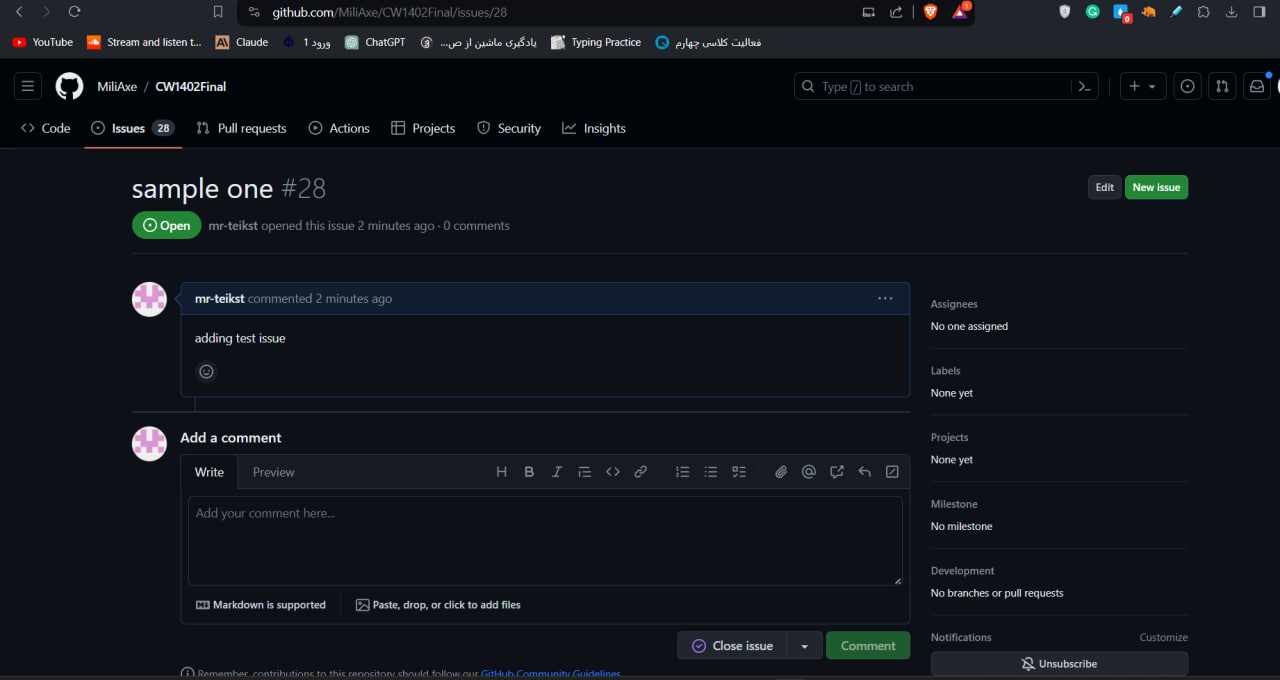
\includegraphics[width=1\textwidth]{photo.jpg}
  \caption{test issue}

\end{figure}



\end{document}
